\documentclass[aspectratio=169,11pt]{beamer}
\usetheme{Madrid}
\usecolortheme{default}
\setbeamertemplate{navigation symbols}{}
\setbeamertemplate{caption}{}
\usepackage{booktabs}
\usepackage{graphicx}
\usepackage{amsmath}

\title[DODVins]{DODVins}
\subtitle{A Data-Oriented MSCKF Pipeline for Predictable Visual-Inertial Odometry\\
\small project walkthrough --- what we built, how we measured it, what it buys}
\author[Shafwan]{Shafwan Safi \and Nikhil Vashisht \and Pranjal Upadhyay}
\institute[]{IISER Bhopal}
\date{}

\begin{document}

%---------------------------------------------------------------
\begin{frame}
  \titlepage
\end{frame}

%---------------------------------------------------------------
\begin{frame}{The question this project answers}
  \begin{itemize}
    \item VIO runs \textbf{per frame, forever}, on hardware that also drives
          control and navigation.
    \item OpenVINS is the reference MSCKF implementation --- but it is built
          for extensibility: heap-allocated per-feature objects,
          \texttt{std::vector} churn, virtual dispatch.
    \item \textbf{Open question:} on a production MSCKF pipeline, how much of
          the per-frame cost is the algorithm, and how much is the
          implementation pattern?
  \end{itemize}
  \vfill
  \centering
  \textbf{DODVins = OpenVINS's estimator, re-implemented under data-oriented
  design constraints, measured against the original.}
\end{frame}

%---------------------------------------------------------------
\begin{frame}{The honest scope, up front}
  \begin{block}{What is unchanged}
    The estimator's \textbf{model}: same MSCKF equations, same state, same
    measurement model as OpenVINS.
  \end{block}
  \begin{block}{What differs --- and we classify every change}
    \begin{itemize}
      \item \textbf{Storage/layout}: fixed-capacity state, feature database
            separating 4-byte keys from payloads, no virtual dispatch.
      \item \textbf{Solver restructures} (numerically equivalent or
            accuracy-gated, each measured separately): square-root-form EKF
            update, one-GEMM $M_a$, measurement compression, $\chi^2$
            early-accept.
      \item \textbf{Initializer}: feature-less solve (from sqrtVINS) ---
            this is where part of the accuracy-difference story comes from.
    \end{itemize}
  \end{block}
\end{frame}

%---------------------------------------------------------------
\begin{frame}{House rules for every line of frame-path code}
  \begin{enumerate}
    \item No variable-sized per-frame objects (no \texttt{new} for features,
          measurements, state; no \texttt{push\_back} churn).
    \item Every capacity fixed at init and \textbf{asserted} --- overflow
          aborts loudly, never corrupts.
    \item No virtual dispatch, no RTTI on the hot path.
    \item Existence-based processing: membership in a pre-filtered table is
          the branch.
    \item Transforms are pure: read inputs, write outputs, no read-back.
  \end{enumerate}
  \vfill
  \small Every optimization was accepted only after DODVins's ten
  trajectories stayed \textbf{bit-identical to its own pre-change output}.
\end{frame}

%---------------------------------------------------------------
\begin{frame}{How we measured --- the rules that make the numbers checkable}
  \begin{itemize}
    \item \textbf{Same transport}: both estimators read the identical rosbag.
    \item \textbf{Same toolchain}: identical Docker container (Ubuntu 20.04,
          ROS1 Noetic, OpenCV 4.2.0, g++ 9.4.0) on both sides --- and on the
          Jetson.
    \item \textbf{Control-tree gate}: two commits built side by side, run on
          identical data, estimate CSVs compared \textbf{byte-for-byte}.
    \item \textbf{Profile, not guess}: two plausible speed hypotheses were
          tested and found wrong; both are reported.
  \end{itemize}
  \vfill
  \small We also measured two confounds that invalidate casually-quoted
  ATEs: \textbf{toolchain choice moves ATE by up to 23\%} (identical code,
  identical data, different OpenCV/g++), transport by 0--5.2\%.
\end{frame}

%---------------------------------------------------------------
\begin{frame}{Result 1 --- accuracy: parity, not superiority}
  \begin{columns}
    \column{0.55\textwidth}
    \small
    \begin{tabular}{lrrr}
      \toprule
      & DODVins & OpenVINS & \\
      \midrule
      Mean ATE (10 seq) & 0.156\,m & 0.158\,m & \\
      Better on & \multicolumn{2}{c}{4 of 10 sequences} & \\
      Drift (1\,s RPE) & \multicolumn{2}{c}{better or equal on 7 of 8 EuRoC} & \\
      \bottomrule
    \end{tabular}

    \vspace{0.4cm}
    \begin{itemize}
      \item MH\_02's gap (0.198 vs 0.162) is an
            \textbf{initialization transient}: DODVins initializes
            $\sim$2\,s earlier from a worse state; drift is nearly identical.
      \item RPE --- not ATE --- reveals this. ATE alone would misattribute
            it to filter quality.
    \end{itemize}
    \column{0.42\textwidth}
    \centering
    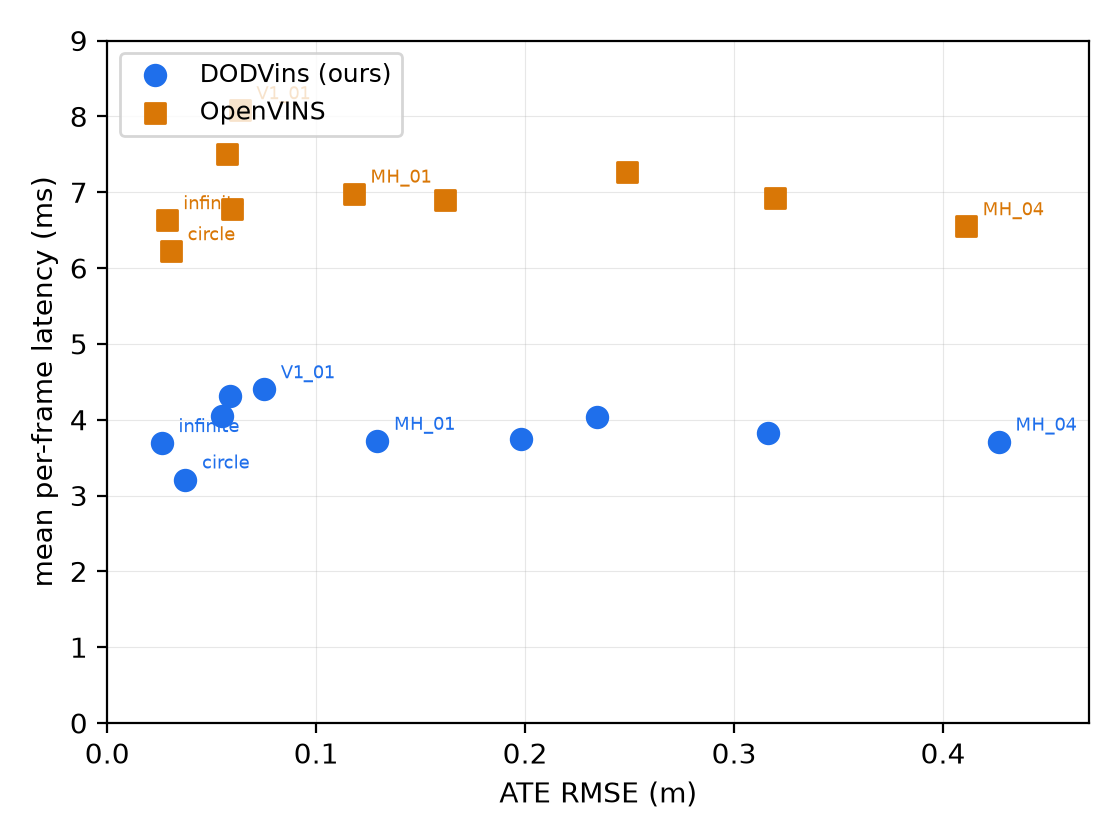
\includegraphics[width=\textwidth]{figs/tradeoff.png}
  \end{columns}
\end{frame}

%---------------------------------------------------------------
\begin{frame}{Result 2 --- speed: consistent, on both axes}
  \begin{columns}
    \column{0.52\textwidth}
    \small
    \begin{tabular}{lcccc}
      \toprule
      & \multicolumn{2}{c}{Wall (s)} & \multicolumn{2}{c}{CPU (s)} \\
      & DOD & OV & DOD & OV \\
      \midrule
      MH\_01 & 14.0 & 29.5 & 29.5 & 44.9 \\
      MH\_04 & 7.7 & 15.7 & 16.3 & 24.3 \\
      circle & 15.7 & 27.6 & 32.5 & 42.8 \\
      \bottomrule
    \end{tabular}
    \vspace{0.3cm}

    \textbf{1.76--2.10$\times$ wall-clock}; 24--34\% less total processor
    time --- the quantity a duty-cycled platform pays for.
    \column{0.46\textwidth}
    \centering
    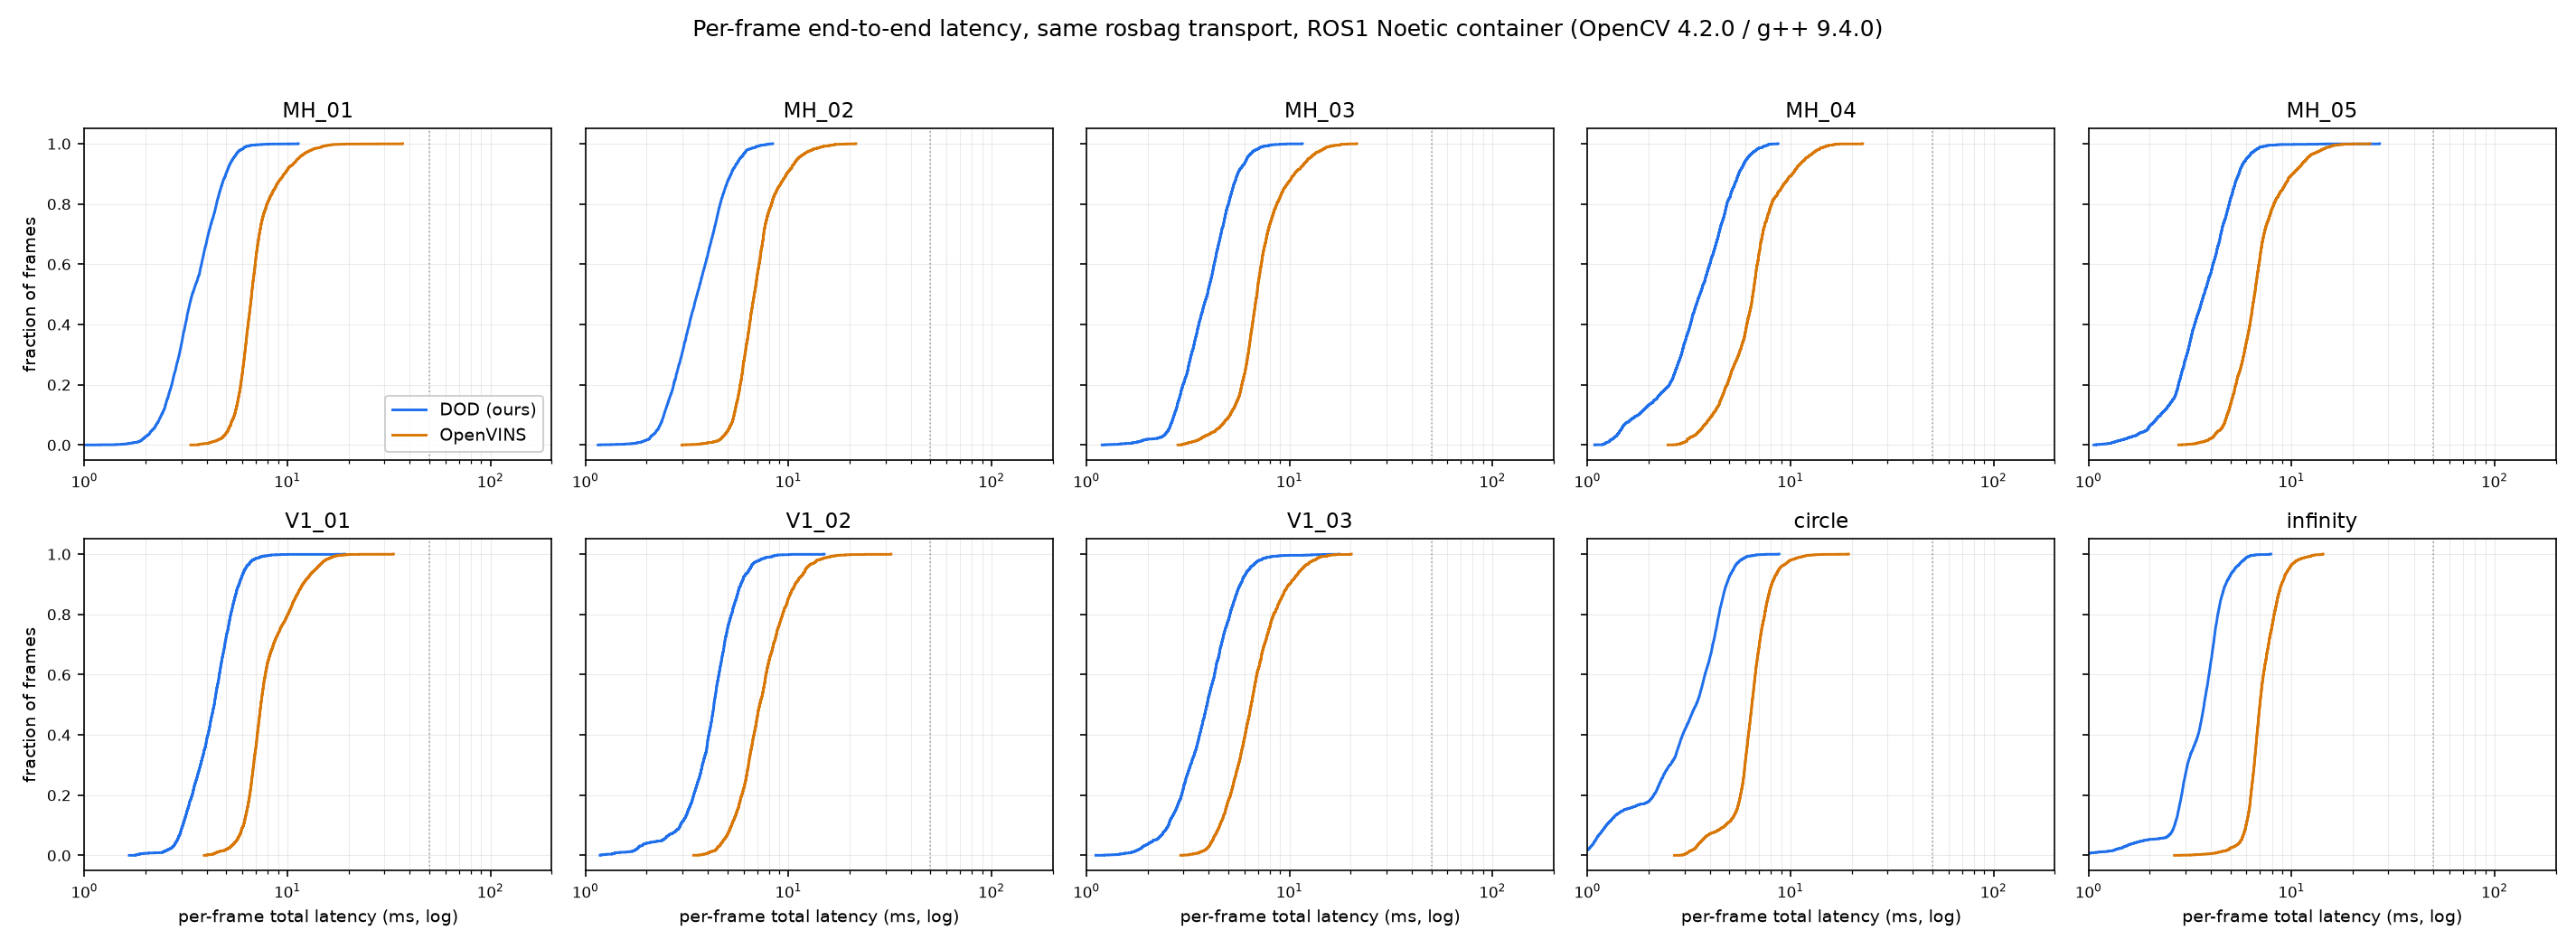
\includegraphics[width=\textwidth]{figs/latency_cdf.png}
  \end{columns}
\end{frame}

%---------------------------------------------------------------
\begin{frame}{Result 3 --- the tail: predictability, our strongest number}
  \begin{itemize}
    \item p99 frame-latency advantage: \textbf{1.64--2.05$\times$} ---
          \emph{exceeds} the mean advantage (1.63--1.85$\times$) on 8 of 10
          sequences.
    \item Worst observed frame: DODVins 8--18\,ms vs.\ OpenVINS
          20--55\,ms. OpenVINS's worst (KAIST circle, 54.8\,ms) blows the
          16\,Hz frame deadline; DODVins never exceeds a third of any
          budget.
  \end{itemize}
  \vfill
  \begin{block}{Why the tail matters}
    Allocator activity and cache misses land in spikes. Winning \emph{more}
    in the tail than in the mean is the signature of a layout win, not an
    arithmetic win.
  \end{block}
\end{frame}

%---------------------------------------------------------------
\begin{frame}{Where the speed comes from --- classified, not assumed}
  \begin{columns}
    \column{0.55\textwidth}
    \small
    \textbf{Solver restructures}: 1.22\,ms/frame attributable
    ($\chi^2$ gate, sqrt-form, GEMM, compression).

    \medskip
    \textbf{Storage/layout}: 0.24\,ms/frame + feature-DB memcpy
    elimination (9{,}556 copies/frame $\rightarrow$ 0).

    \medskip
    \textbf{Mixed} (row 8, 1.97\,ms): arithmetic and placement
    restructured together --- cannot be split honestly.

    \column{0.43\textwidth}
    \begin{block}{Honest scaling example}
      The square-root EKF update: 0.29\,ms/frame ($\approx$8\% of the
      total gain). Its primary contribution is \textbf{correctness} ---
      the dense form drives covariance diagonals negative and aborts
      MH\_01 at $t{=}16$\,s.
    \end{block}
  \end{columns}
  \vfill
  \small Every row of the ablation was measured with all ten trajectories
  bit-identical before and after.
\end{frame}

%---------------------------------------------------------------
\begin{frame}{"Allocation-free" --- what we claim, precisely}
  \begin{columns}
    \column{0.55\textwidth}
    DHAT attribution, 12\,s of MH\_01 (777{,}007 blocks, 1.89\,GB):
    \begin{itemize}
      \item 59\% --- OpenCV KLT tracker internals (not ours)
      \item 19\% --- DODVins estimator: \textbf{bounded Eigen workspaces},
            137 blocks / 3.8\,MB per frame in \texttt{EKFUpdate}
      \item 15\% --- one-time library startup; 3\% --- dataset I/O
    \end{itemize}
    \column{0.43\textwidth}
    \begin{block}{Precise claims}
      \begin{itemize}
        \item Propagation path: \textbf{zero} allocations (unit-test
              asserted).
        \item No per-feature / per-measurement heap objects, ever.
        \item Working set does not grow with sequence length.
      \end{itemize}
      We do \emph{not} claim the dense update workspaces are
      allocation-free --- we measured them instead.
    \end{block}
  \end{columns}
\end{frame}

%---------------------------------------------------------------
\begin{frame}{Result 4 --- Jetson Orin Nano: it transfers, narrower}
  \begin{itemize}
    \item Same toolchain container on aarch64 --- \textbf{ISA is the only
          variable}.
    \item Median latency: 27--35\,ms vs OpenVINS 34--47\,ms
          (\textbf{1.16--1.61$\times$}); faster on all ten sequences.
    \item Margin \emph{narrows}: p99 advantage is smaller than on x86
          (plausible cause: LPDDR5 bandwidth --- untested, stated as such).
    \item Peak RSS: \textbf{184--199\,MB flat} vs OpenVINS 98--179\,MB
          variable. We trade higher average utilization for a bounded
          working set --- owned, not hidden.
  \end{itemize}
\end{frame}

%---------------------------------------------------------------
\begin{frame}{Result 5 --- TUM VI: the untuned independent test}
  \begin{columns}
    \column{0.52\textwidth}
    \begin{itemize}
      \item Third dataset family, first fisheye camera
            (Kannala-Brandt~4 --- the pipeline already had the model).
      \item \textbf{Only calibration adapted}; every estimator knob is the
            marked EuRoC placeholder.
      \item All six room sequences initialize and converge.
      \item Mean ATE \textbf{0.062 vs 0.063\,m} (OpenVINS, same Kalibr
            release): parity, DODVins better on 3 of 6.
    \end{itemize}
    \column{0.46\textwidth}
    \centering
    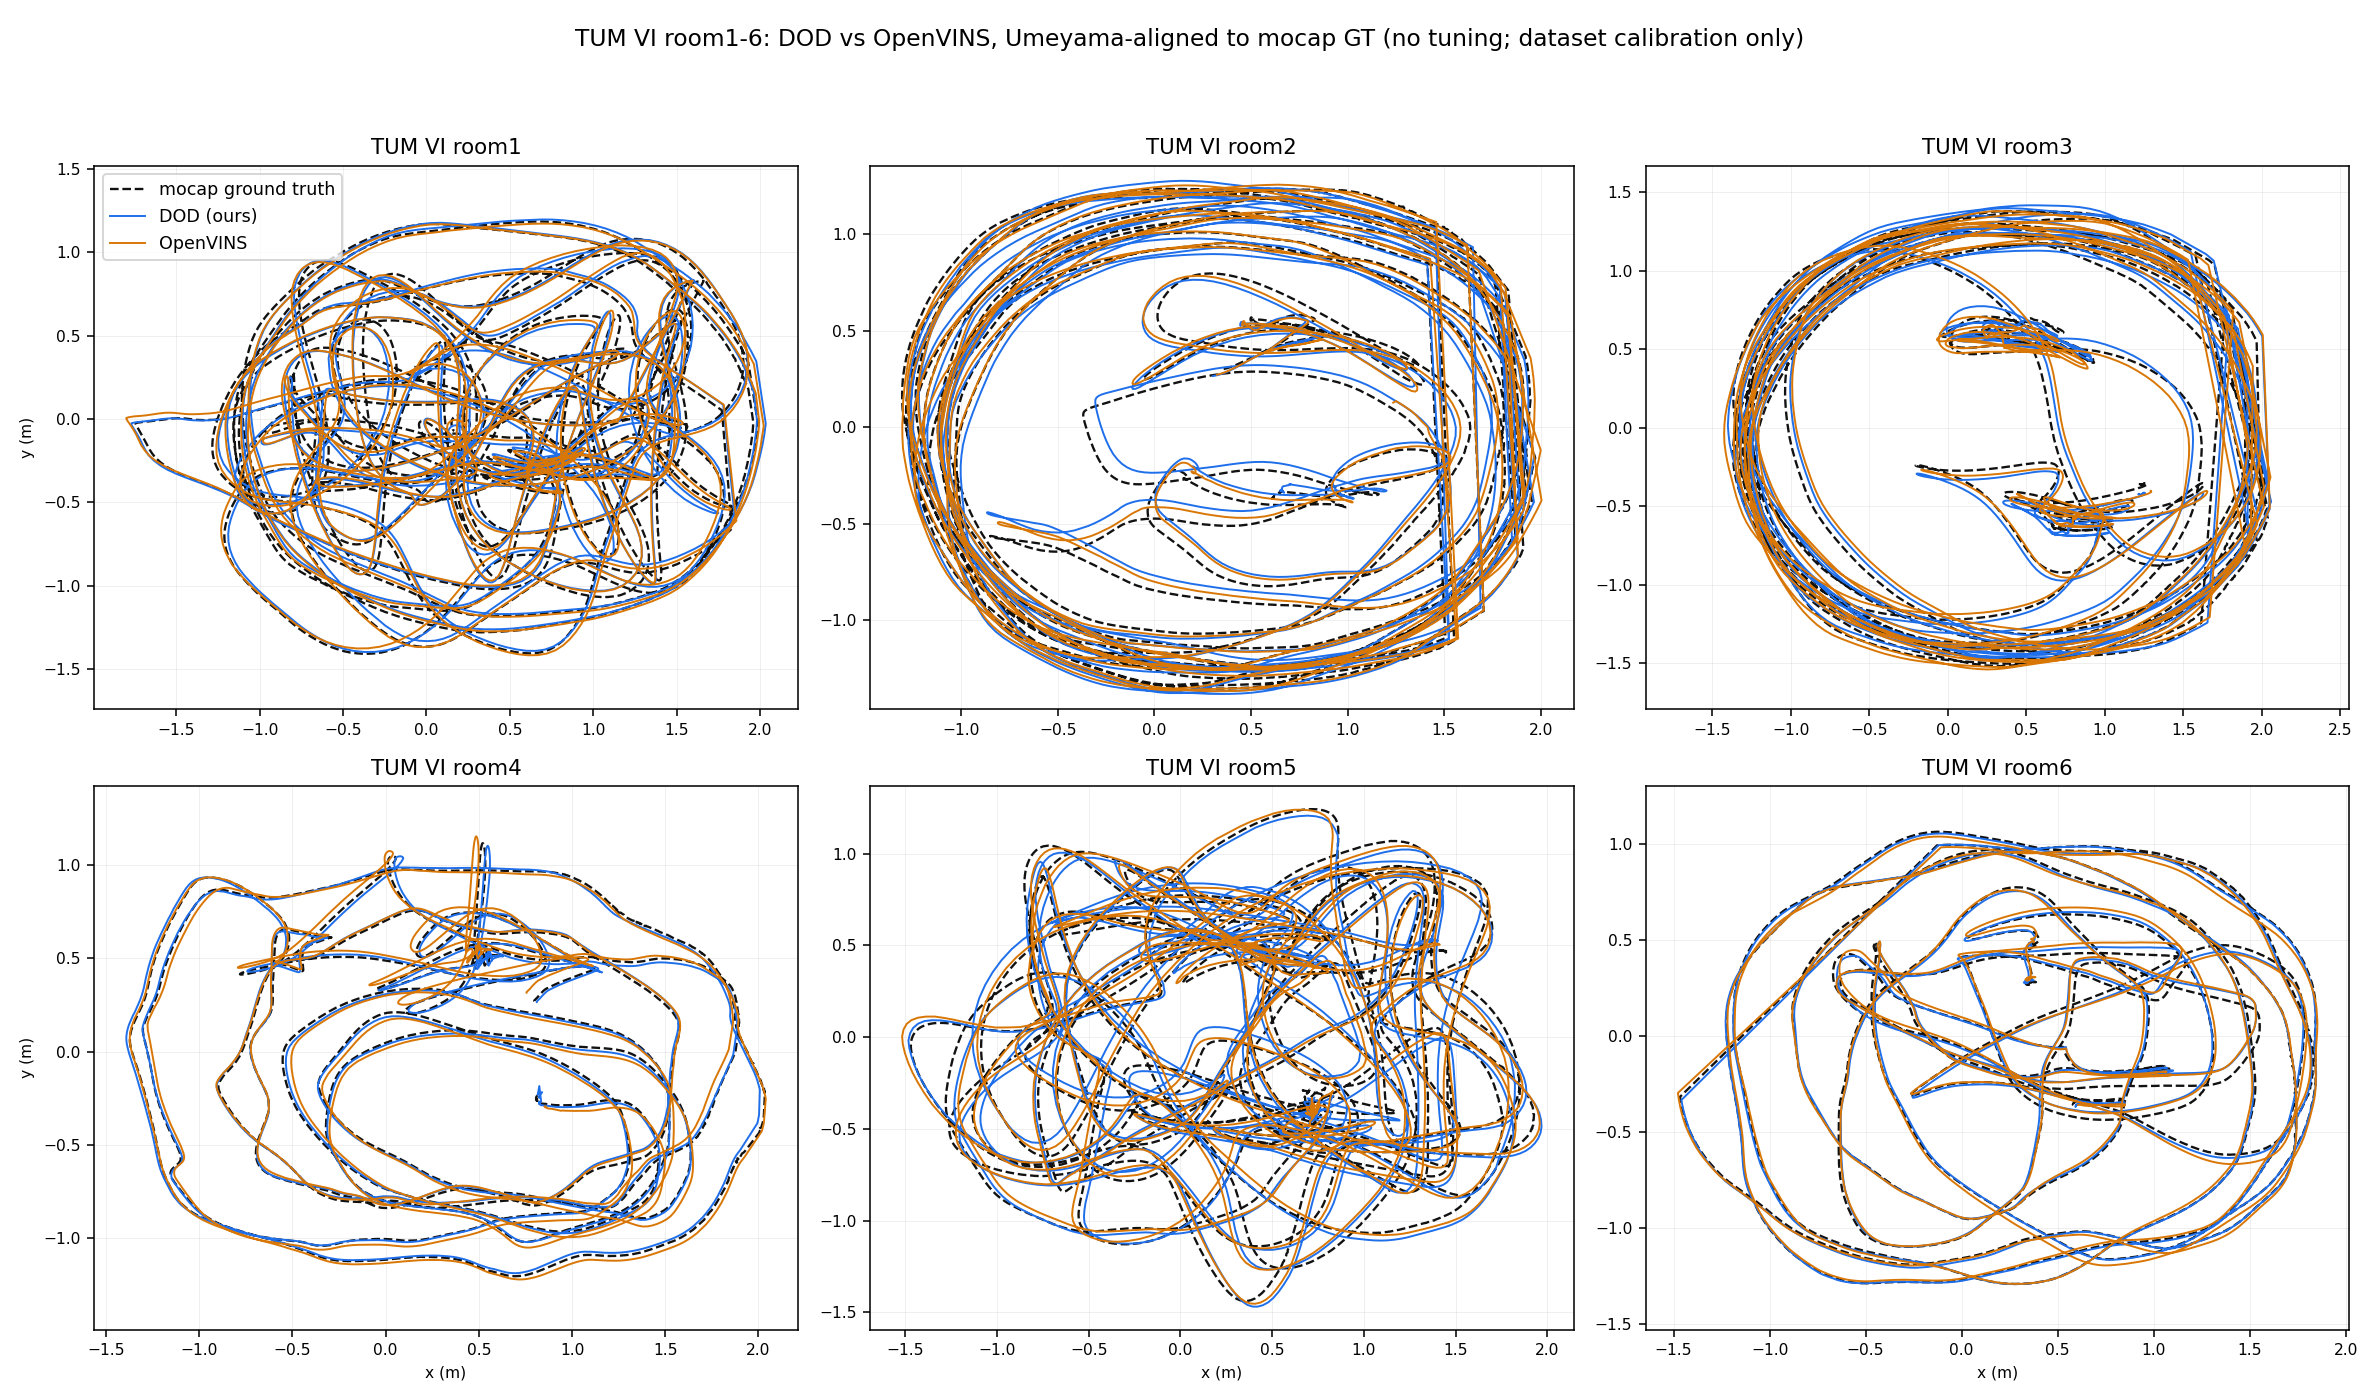
\includegraphics[width=\textwidth]{figs/tumvi_all_rooms.png}
  \end{columns}
\end{frame}

%---------------------------------------------------------------
\begin{frame}{Result 6 --- high-altitude outdoor: where MSCKF breaks}
  \begin{columns}
    \column{0.55\textwidth}
    \small
    \begin{tabular}{lrrr}
      \toprule
      Alt & DODVins ($\sigma{=}1$) & tuned $\sigma$ & OpenVINS \\
      \midrule
      40\,m  & 12.81 & 12.81 & \textbf{4.19} \\
      60\,m  & 1367.7 $\times$ & 48.3 & \textbf{12.22} \\
      80\,m  & 56303 $\times$ & \textbf{23.2} & 145059 $\times$ \\
      100\,m & 94897 $\times$ & 110.3 & \textbf{57.2} \\
      \bottomrule
    \end{tabular}
    \column{0.43\textwidth}
    \small Outdoor UAV, 30\,cm baseline, 40--100\,m altitude:
    depth/baseline ratio 130--330.
    \begin{itemize}
      \item \textbf{No shipped config covers the envelope} --- both
            pipelines are one inherited constant from divergence.
      \item DODVins latency outdoors unchanged: 2.6--3.9\,ms median.
    \end{itemize}
  \end{columns}
\end{frame}

%---------------------------------------------------------------
\begin{frame}{What this does not claim}
  \begin{itemize}
    \item \textbf{No estimator novelty} --- every equation is OpenVINS's;
          the contribution is implementation + measurement.
    \item \textbf{Accuracy superiority} --- parity; worse on 6 of 10.
    \item \textbf{Lower memory} --- higher average RSS; the claim is
          \emph{bounded}, not minimal.
    \item \textbf{Full allocation-freedom} --- propagation is; the update's
          dense workspaces are measured, not hidden.
    \item Untuned-on-TUM-VI means the numbers there are the inherited
          configuration's, not the pipeline's best.
    \item Jetson thermal/frequency state uncontrolled (limitations say so).
  \end{itemize}
\end{frame}

%---------------------------------------------------------------
\begin{frame}{For a practitioner}
  \begin{itemize}
    \item Desktop x86: same MSCKF trajectories for $\sim$half the
          wall-clock and a quarter to a third less processor time, with a
          frame-latency tail inside the sensor's budget.
    \item Jetson-class SoC: same directions, narrower margins.
    \item Estimator must share compute with control/navigation? DODVins
          frees that share \textbf{without changing a filter equation}.
    \item Relying on loop closure or tight memory ceilings? Weigh the
          recorded trade-offs first.
    \item And regardless of pipeline: quote ATEs with transport
          \emph{and} toolchain, or they cannot be reproduced.
  \end{itemize}
\end{frame}

%---------------------------------------------------------------
\begin{frame}{Reproducibility}
  \begin{itemize}
    \item Public repo: \texttt{github.com/Shafwansafi06/vio\_pipeline\_cpp}
          (tag \texttt{v0.1.0} = submission snapshot).
    \item \texttt{artifact/README.md}: every paper number $\rightarrow$ its
          archived run or its script.
    \item Harnesses included: x86 latency/RSS matrix, Orin matrix,
          control-tree byte-compare (the method behind every optimization
          claim).
    \item Paper: \texttt{paper/main.pdf} --- 8 pages, every number traced.
  \end{itemize}
\end{frame}

%---------------------------------------------------------------
\begin{frame}{Summary}
  \begin{enumerate}
    \item Same MSCKF math, data-oriented implementation:
          \textbf{1.76--2.10$\times$ faster} at accuracy parity.
    \item The tail (p99) improves \emph{more} than the mean --- the layout
          signature.
    \item Every optimization individually measured, classified
          (solver vs storage), and gated bit-identically.
    \item Transfers to Jetson (narrower), untuned to TUM VI (parity),
          honestly broken at high altitude like everything else --- with
          the failure diagnosed by counters, not guesses.
    \item Two benchmarking confounds (toolchain 23\%, transport 5\%)
          measured, so our numbers --- and anyone else's --- can be
          reproduced.
  \end{enumerate}
  \vfill
  \centering\small Questions welcome --- every number has a ticket behind it.
\end{frame}

\end{document}
